\tp{\'Etude de piles}


\Large


%\vressort{1}
\vressort{3}

\objectifs{
\normalsize
\item d�terminer exp�rimentalement la polarit� d'une pile
\item mesurer la force �lectromotrice d'une pile
\item �tudier l'influence de la concentration de l'un des cations
m�talliques sur la force �lectromotrice.
}

\vressort{1}


\materiel{
\normalsize
\item solution � $c = 0,1~mol.L^{-1}$ de
        \begin{itemize}
        \item sulfate de cuivre
        \item nitrate de fer
        \item nitrate de plomb
        \end{itemize}

\item solution de sulfate de cuivre $c = 1~mol.L^{-1}$
\item solution de sulfate de zinc de concentrations : $1~mol.L^{-1}$ ;
$0,1~mol.L^{-1}$ ; $0,01~mol.L^{-1}$
\item �lectrodes m�talliques de cuivre, zinc, fer, plomb
\item ponts salins
\item multim�tre
}


\vressort{3}

\section{Manipulations}

\subsection{R�alisation des piles}

\begin{enumerate}

\item R�aliser les trois demi-piles :
  \begin{itemize}
  \item $Fe^{2+} / Fe$
  \item $Pb^{2+} / Pb$
  \item $Zn^{2+} / Zn$
  \end{itemize}
  ($c = 0,1~mol.L^{-1}$).

\item Associer chacunes d'elles � la demi-pile $Cu^{2+} / Cu$.

\item D�terminer la polarit� de chacune des piles r�alis�es.

\item Mesurer la force �lectromotrice de chacune des piles.

\item Pr�ciser pour chaque pile les demi-�quations �lectroniques et
l'�quation de fonctionnement.

\item \emph{Remarque :}�bien d�caper les lames m�talliques avant
chaque utilisation.

%\item 
\end{enumerate}

\vressort{1}

\normalsize

%\begin{tabularx}{\linewidth}{|X|X|X|X|X|X|}
%\begin{tabularx}{\linewidth}{|*{6}{X|}}
\begin{tabularx}{\linewidth}{|*{6}{>{\centering}X|}}
\hline
Pile & \'Electrode $+$ & \'Electrode $-$ & fem ($V$) & Demis-�quations
& \'Equation \tbnl
\rule[-0.5cm]{0cm}{1cm}
        &       &       &       &       & \tbnl
\rule[-0.5cm]{0cm}{1cm}
        &       &       &       &       & \tbnl
\rule[-0.5cm]{0cm}{1cm}
        &       &       &       &       & \tbnl
\end{tabularx}

\Large


\newpage


\subsection{Influence de la concentration $[Zn^{2+}]$ sur la force
�lectromotrice d'une pile Daniell}


La pile Daniell est constitu�e des deux demi-piles $Zn^{2+} / Zn$ et
$Cu^{2+} / Cu$.


% sch�ma
\begin{center}
\begin{figure}[H]
\caption{Pile Daniell}
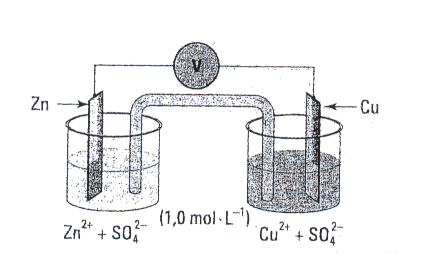
\includegraphics[width=8cm]{oxydo_reduction/tp_piles/pile_daniell.png.eps}
\end{figure}
\end{center}

R�aliser trois piles avec une solution de sulfate de cuivre $c =
1~mol.L^{-1}$ et une solution de sulfate de zinc :

\begin{itemize}
\item $c_1 = 1~mol.L^{-1}$
\item $c_2 = 0,1~mol.L^{-1}$
\item $c_3 = 0,01~mol.L^{-1}$
\end{itemize}


\vspace{1cm}


\normalsize

%\begin{tabularx}{\linewidth}{|X|X|X|X|}
\begin{tabularx}{\linewidth}{|*{4}{>{\centering}X|}}
\hline
\rule[-0.5cm]{0cm}{1cm}
$[Cu^{2+}]$ ($mol.L^{-1})$ & $1,0$ & $1,0$ & $1,0$  \tbnl
\rule[-0.5cm]{0cm}{1cm}
$[Zn^{2+}]$ ($mol.L^{-1})$ & $1,0$ & $0,1$ & $0,01$ \tbnl
\rule[-0.5cm]{0cm}{1cm}
$f.e.m.$ ($V$)          &       &       &        \tbnl
\end{tabularx}

\Large



\section{Conclusions}

\begin{enumerate}
\item Quel type de r�action se produit sur l'�lectrode positive ?
\item Quel type de r�action se produit sur l'�lectrode n�gative ?
\item Quel est l'influence de la concentration en cation m�tallique
sur la f.e.m. ?
\end{enumerate}

\normalsize

